\section{Кросс-валидация}
Чтобы получить более реалистичную оценку ошибки предсказания, мы хотели бы иметь тестовую выборку, отличную от нашей обучающей выборки. В идеале это могли бы быть новые данные из той же генеральной совокупности, из которой была взята наша первоначальная выборка. В нашем примере это количество часов, которое носилось устройство и количество оставшегося в нем гормона, скажем для $m$ новых устройств. Если бы у нас были эти новые данные, $(z_{1}^{0}, y_{1}^{0}),\ldots, (z_{m}^{0},y_{m}^{0})$, мы вычислили бы значения предсказаний $\what{y_{i}}^{0}$ из таблицы $(9.3)$:
\begin{equation}
\what{y_{i}}^{0} = \what{\beta_{j}}^{0} + \what{\beta_{1}}^{0}z_{i}^{0},
\end{equation}
(где $j = A, B$ или $C$ в зависимости от партии) и среднюю сумму квадратов разности:
\begin{equation}
\summ{1}{m} \frac{(y_{i}^{0} - \what{y_{i}}^{0})^{2}}{m}.
\end{equation}
Эта величина оценивает, насколько в среднем наш прогноз $\what{y_{i}}^{0}$ отличается от фактического значения $y_{i}^{0}$. 

Обычно дополнительные данные недоступны по причинам трудозатратности или стоимости. Чтобы решить эту проблему, кросс-валидация использует одну часть имеющихся данных для построения модели, а другую часть для ее тестирования. При больших объемах данных обычной практикой является разделение данных на две равные части. Когда объем данных не большой, как в случае с данными о гормонах, k-fold кросс-валидация позволяет более эффективно использовать доступные данные. Процедура показана в алгоритме $17.1.$
\begin{algorithm}
\caption{$k$-fold кросс-валидация}
1. Разделите данные на $K$ частей примерно равного размера.

2. Постройте модель по $K - 1$ частям данных и вычислите ошибку предсказания построенной модели на предсказании для k-й части данных, которая не участвовала в построении модели.

3. Выполните эти два шага для k = 1, 2, ... $K$ и сложите $K$ оценок ошибок предсказания.
\end{algorithm}

Далее рассмотрим $k$-fold кросс-валидацию подробнее. Предположим, мы разбиваем данные на $K$ частей. Пусть $k(i)$ --- это часть, которая содержит $i$ - ое наблюдение. Обозначим через $\what{y}_{i}^{-k(i)}$ предсказание для $i$ - го наблюдения, которое было вычисленно по данным с удалением $k(i)$ - ой части. Тогда оценка ошибки предсказания полученная с помощью кросс-валидации будет равна:
\begin{equation}
\tx{CV} = \frac{1}{n} \summ{i = 1}{n} (y_{i} - \what{y}_{i}^{-k(i)})^{2}.
\end{equation}
Часто выбирается $k = n$, что приводит к <<leave-one-out>> кросс-валидации. Строим модель без учета $i$-го наблюдения, а затем используем ее для его предсказания, обозначим результат предсказания $\what{y}_{i}^{-i}$. Мы делаем так для каждого наблюдения, а затем вычисляем среднюю сумму квадратов полученную с помощью кросс-валидации $\tx{CV} = \summ{i = 1}{n} \frac{(y_{i} - \what{y}_{i}^{-i})^{2}}{n}$.

Мы использовали leave-one-out кросс-валидацию к данным по гормонам: значение CV оказалось равным $3.09$. Для сравнения, средняя остаточная квадратичная ошибка (17.3) равна $2.20$, таким образом, она занижает значение ошибки предсказания примерно на $29\%$. На рисунке 17.2 показан график обычных остатков $y_{i} - \what{y}_{i}$ (кружки) и график остатков полученных с помощью кросс-валидации $y_{i} - \what{y}_{i}^{-i}$ (звездочки). Обратите внимание, что для каждого наблюдения, значения остатков полученных с помощью кросс-валидации или больше (по абсолютной величине) обычных остатков или равны им. 
\begin{figure}[h]
\center{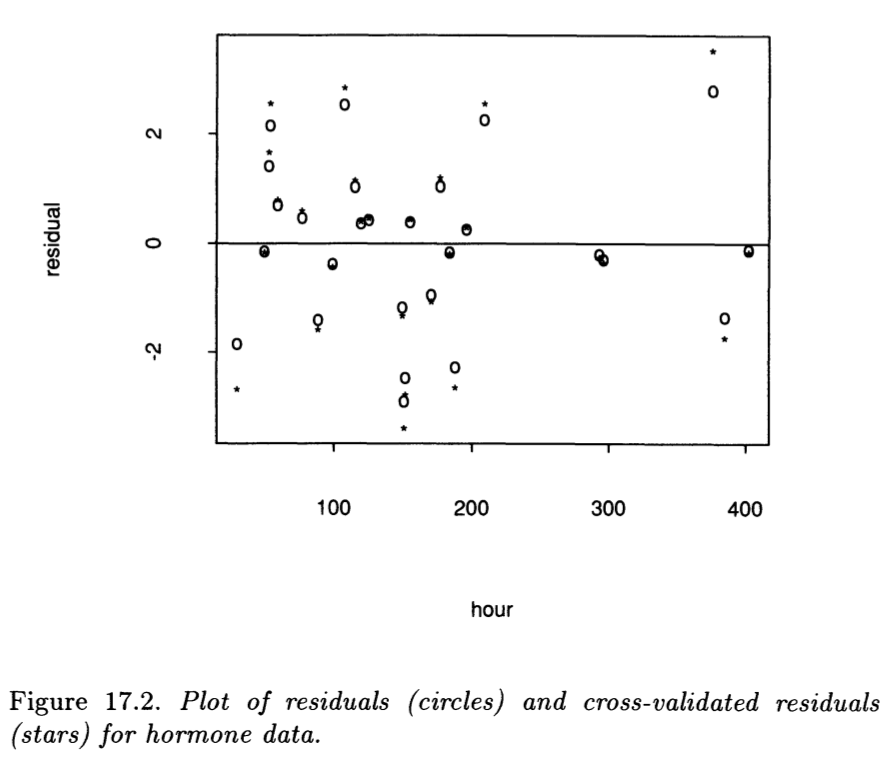
\includegraphics[width=1 \linewidth]{17/f17.2.png}}
\end{figure}

Далее мы можем посмотреть на разбивку $\tx{CV}$ по партиям: средние значения равны $2.09$, $4.76$ и $2.43$ для парти $A$, $B$ и $C$, соответственно. Следовательно, сложнее предсказать значения для устройств из партии $B$, нежели для устройств из партий $A$ и $C$. 

Кросс-валидация, как было описано выше, требует обучения всей модели \textit{$n$ раз}. В общем, это неизбежно, но для аппроксимации методом наименьших квадратов возможен более рациональный способ.


